\documentclass[11pt]{article}
\usepackage[margin=1in]{geometry}
\usepackage{amsmath,amssymb,amsthm,booktabs,hyperref,tikz,microtype,xcolor}
\hypersetup{colorlinks=true,linkcolor=blue!55!black,urlcolor=blue!55!black,citecolor=blue!55!black,
 pdftitle={Four Black Cells Force an Outgoing Highway: A Sharp Half-Plane Threshold for Langton's Ant},pdfauthor={Hao Ke}}
\newtheorem{theorem}{Theorem}
\newtheorem{lemma}[theorem]{Lemma}
\newtheorem{corollary}[theorem]{Corollary}
\newcommand{\Z}{\mathbb Z}
\newcommand{\N}{\mathbb N}
\newcommand{\HH}{\mathcal H}
\title{Four Black Cells Force an Outgoing Highway:\\A Sharp Half-Plane Threshold for Langton's Ant}
\author{Hao Ke}
\date{15 October 2026}
\begin{document}
\maketitle
\begin{abstract}
Four initially black cells suffice to keep the classical Langton ant forever
in a prescribed half-plane and launch its standard period-104 highway. Four
is optimal: starting at the boundary and facing inward, every colouring with
at most three black cells in that half-plane exits within 918 updates, and
this time bound is sharp. The lower bound covers arbitrary cell coordinates
through a finite first-contact enumeration. An explicit four-cell seed has a
certified standard highway from update 182; exact colour-parity identities
establish its entire infinite tail. We then show that every finite-support
initial state admits an effective extension by exactly four remote black
cells that preserves any prescribed finite observed trajectory and forces
standard-highway behaviour. The construction joins the original trajectory
at its first exit from a protected square, while retaining its complete
physical history. Analytic coverage and coupling arguments are accompanied
by reproducible finite certificates and separately implemented checks.
\end{abstract}

\section{A sharp outgoing interface}
A local pattern can determine the ant's eventual motion while leaving an
arbitrarily long initial observation unchanged. We construct such a pattern
using four black cells in a half-plane. The supporting line separates its
entire future from any configuration on the other side, making the pattern
an outgoing interface for arbitrary finite histories. A matching lower bound
shows that four cells are necessary for this one-sided interface.

A colouring is a set $B\subseteq\Z^2$ of black cells; $p$ and $h$ denote the
ant's position and cardinal heading. On an update, the ant turns left on
black and right on white, toggles the current cell, and moves one unit in the
new heading. Let $(B_t,p_t,h_t)$ be the state before update $t$, and define
its observation as
\[
 O_t=(p_t,h_t,\mathbf1_{B_t}(p_t)).
\]
The half-plane result permits arbitrary exterior colouring. Finite support
is required for the exterior-completion theorem.

Put $\HH_+=\{(x,y):x\ge0\}$. A \emph{one-sided port} is a finite black seed
in $\HH_+$ whose trajectory, from $(0,0)$ facing east, remains in $\HH_+$
forever. The \emph{standard P104 trace} is the fixed blank-orbit 104-turn word
at update 9977, repeated forever, with a lattice translation, quarter-turn
rotation and cyclic phase allowed. Positions, headings and read colours are
part of this trace; black cells away from its future path remain in the state.

\begin{theorem}[Sharp half-plane escape]\label{th:threshold}
Start at $(0,0)$ facing east. For every initial colouring with at most three
black sites in $\HH_+$, regardless of the colours in $x<0$, the first-exit time
\[
 \tau=\min\{t\ge0:(p_t)_x<0\}
\]
satisfies $\tau\le918$. Equality holds for
$B_* = \{(0,-1),(2,1),(3,3)\}$ with all other cells white.
\end{theorem}

\begin{theorem}[A four-cell outgoing port]\label{th:port}
For $G=\{(0,-1),(1,1),(1,3),(2,2)\}$ and initial pose $(0,0),E$, every
$p_t$ lies in $\HH_+$. At update 182 the position is $(5,1)$, the heading is
$E$, and there are 36 black cells. The entire future from this state is the
standard P104 trace, with drift $(2,2)$ per 104 updates. Consequently four
is the minimum black-cell cardinality of a one-sided port.
\end{theorem}

\begin{figure}[ht]
\centering
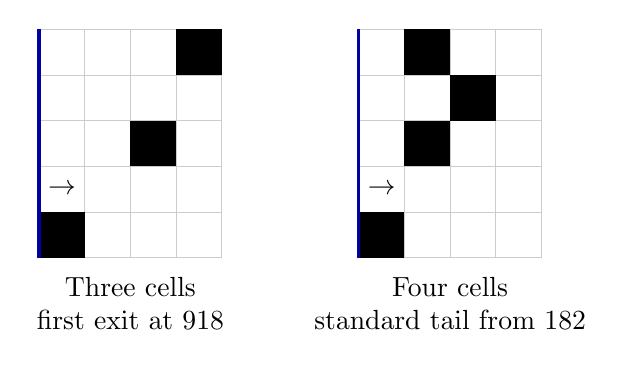
\begin{tikzpicture}[scale=.58]
\begin{scope}
 \draw[xshift=-.5cm,yshift=-.5cm,step=1,gray!40,very thin] (0,-1) grid (4,4);
 \foreach \x/\y in {0/-1,2/1,3/3}
  {\fill (\x-.5,\y-.5) rectangle (\x+.5,\y+.5);}
 \draw[very thick,blue!65!black] (-.5,-1.5)--(-.5,3.5);
 \node at (0,0) {$\rightarrow$};
 \node[align=center] at (1.5,-2.5) {Three cells\\first exit at 918};
\end{scope}
\begin{scope}[xshift=7cm]
 \draw[xshift=-.5cm,yshift=-.5cm,step=1,gray!40,very thin] (0,-1) grid (4,4);
 \foreach \x/\y in {0/-1,1/1,1/3,2/2}
  {\fill (\x-.5,\y-.5) rectangle (\x+.5,\y+.5);}
 \draw[very thick,blue!65!black] (-.5,-1.5)--(-.5,3.5);
 \node at (0,0) {$\rightarrow$};
 \node[align=center] at (1.5,-2.5) {Four cells\\standard tail from 182};
\end{scope}
\end{tikzpicture}
\caption{The sharp three-cell witness $B_*$ and the four-cell port $G$.
Cell coordinates refer to square centres. The ant starts at $(0,0)$ facing
east; the blue line separates columns $-1$ and $0$.}
\end{figure}

The port gives a completion theorem for any finite initial state. The
preserved object is the observed trajectory: the four extra black cells are
present in the modified colouring from time zero.

\begin{theorem}[Four-cell exterior completion]\label{th:extension}
Let $X=(B,p,h)$ have finite black support. Given a finite protected set $K$,
an integer $T\ge0$, and any axis-aligned square $Q$ containing $B$, $K$ and
the $\ell^\infty$ ball of radius $T$ about $p$, one can compute a four-element
set $A\subset\Z^2\setminus Q$ such that the evolution of
$X^+=(B\cup A,p,h)$ satisfies
\[
 O_t(X^+)=O_t(X)\qquad(0\le t<T)
\]
and eventually has the standard P104 trace. If $Q$ has $n$ cells per side,
that trace starts by update $8n3^n+183$.
\end{theorem}

The proof has three parts. First-contact branching reduces the unrestricted
three-cell problem to a finite family. Exact parity then certifies the
four-cell infinite trajectory. Finally, the port is placed beyond the first
exit from $Q$, so its future avoids every earlier black cell.

\section{First-contact coverage and the sharp bound}
For a finite seed $S\subset\HH_+$, let $t(S)$ be its first exit, when finite.
Let $V(S)$ contain each cell whose first read before $t(S)$ is white. Define
\[
 \mathcal F_0=\{\varnothing\},\qquad
 \mathcal F_{j+1}=\{S\cup\{q\}:S\in\mathcal F_j,\ q\in V(S)\}.
\]
This construction uses the cells reached by exact trajectories, so the input
coordinates require no bounding box.

\begin{lemma}[First-contact coverage]\label{lem:coverage}
If every member of $\mathcal F_0,\ldots,\mathcal F_k$ exits in finite time,
every colouring with at most $k$ black sites in $\HH_+$ exits by
$M=\max\{t(S):S\in\mathcal F_j,\ 0\le j\le k\}$.
\end{lemma}
\begin{proof}
Suppose an actual trajectory stays in $\HH_+$ through time $M$. Start with
$S=\varnothing$, a subset of its initially black sites in $\HH_+$. If the
actual trajectory agrees with the trajectory from $S$ until its exit, it
exits by $M$, contrary to the supposition. Otherwise take the first differing
read. All earlier reads and writes agree; hence their colour difference at
this cell is its initial colour difference. The cell belongs to the actual
initial black set but not to $S$. It was never read earlier, since an earlier
read would already have revealed that difference. Thus it belongs to $V(S)$,
and adjoining it gives a member of the next family, still a subset of the
actual black set. Each repetition adds a distinct black cell. At most $k$
repetitions exhaust that set, after which a further differing read is
impossible. Cells in $x<0$ are not read before the first exit.
\end{proof}

Exact enumeration gives the complete families:
\begin{center}
\begin{tabular}{rrr}
\toprule
$j$ & $|\mathcal F_j|$ & $\max t(S)$\\
\midrule
0 & 1 & 2\\
1 & 2 & 38\\
2 & 20 & 106\\
3 & 261 & 918\\
\bottomrule
\end{tabular}
\end{center}
The 284 records specify each seed, exit time and exit position. A verifier
reconstructs all first-visit sets, checks equality with the next family,
and replays every exit. A separate implementation branches on the initial
colour at each first visit, with a three-black budget, and obtains the same
maximum. The two enumerations have different counts because the online tree
identifies redundant or unread black choices.

For $B_*$, the ant is at $(0,7)$ facing south before update 917, reading
white. The resulting right turn moves it to $(-1,7)$ at time 918. The finite
certificates and Lemma~\ref{lem:coverage} prove Theorem~\ref{th:threshold}.
A check that reaches its safety cap fails; it never treats an unfinished
trajectory as evidence of escape or eternal residence.

\section{Certifying the outgoing infinite trace}
Exact replay of $G$ for 182 updates gives the endpoint in
Theorem~\ref{th:port}, with every prefix position in $\HH_+$. Let $B'$ be
its complete 36-cell black set. Fix the standard word $w$, obtained by
replaying the blank ant from $(0,0),N$ to time 9977 and reading its next
104 turns. The same word, started from $(5,1),E$, restores its heading and
has drift $d=(2,2)$.

Write $q_i$ for the \emph{absolute} pre-update position in phase
$i\in\{0,\ldots,103\}$ of this proposed block. Its infinite motion plan
reads $q_i+kd$ at time $104k+i$, and the $x$-coordinates of the $q_i$ range
from 4 through 9. It therefore suffices to verify the read colour at every
such position and time.

\begin{lemma}[Finite parity test for an infinite trace]\label{lem:parity}
Let a finite word $w$ restore its heading with nonzero drift $d$, and let
$q_i$ be its phase positions. From a finite initial black set $B'$, the
proposed repeated trace is an actual ant trajectory if and only if, for every
phase $i$ and integer $k\ge0$,
\begin{equation}\label{eq:parity}
 \mathbf1_{B'}(q_i+kd)\ \oplus\
 \bigl|\{(j,s):q_j-q_i=sd,\ 0\le s\le k,
                 \ s>0\ \text{or}\ (s=0\text{ and }j<i)\}\bigr|\bmod2
 =\mathbf1_{\{w_i=L\}}.
\end{equation}
It is sufficient to check $k=0$, every nonnegative overlap threshold $s$,
and every nonnegative initial-black hit epoch and its successor.
\end{lemma}
\begin{proof}
A previous read at $q_j+\ell d$ affects the proposed read at $q_i+kd$
exactly when $q_j-q_i=(k-\ell)d$. Setting $s=k-\ell$, its time is earlier
exactly when $s>0$, or $s=0$ and $j<i$; nonnegative $\ell$ gives $s\le k$.
Each preceding read toggles the cell once, giving the left side of
\eqref{eq:parity}. Necessity follows from the rule, and sufficiency follows
by induction on chronological time.

For fixed $i,j$, nonzero $d$ gives at most one integer $s$, whose parity
contribution starts at that threshold. Each initial black cell lies on the
phase ray at at most one epoch $k$; its contribution is present only there,
so both $k$ and $k+1$ are breakpoints. Between consecutive breakpoints every
term is constant. The last breakpoint also represents the final unbounded
interval. These finitely many tests therefore cover every $k\ge0$.
\end{proof}

For the port endpoint, the test uses 170 phase/epoch evaluations and accepts
$w^\omega$. Applied independently to the actual blank endpoint, it certifies
that $w$ is the standard infinite word. The prefix guard, the phase-position
range and the positive $x$-drift now prove the port stays in $\HH_+$ forever.
Together with Theorem~\ref{th:threshold}, this proves four-cell optimality.

An additional check uses chronological visits to each physical cell, as in
the periodic-realisability criterion of Jillhewar~\cite{jillhewar2026}.
Partition phases modulo the full group $\Z d$, and write
$q_i=a+\ell_i d$ in each class. The cell $a+nd$ is visited at times
$104(n-\ell_i)+i$ for all $\ell_i\le n$. At these times the prescribed
colours must alternate, beginning with its initial colour. The visit list
changes only when $n$ passes a phase level $\ell_i$; initial black cells add
singleton changes. Checking the resulting finite intervals, including the
last, is another exact all-future verification. The independent audit checks
40 cell intervals in 22 translation classes, both for the port and the
blank reference.

The smallest black set required on the port's future read set consists of
13 cells:
\begin{align*}
 K_0=\{&(4,3),(4,4),(5,1),(5,5),(5,6),(5,7),\\
       &(6,1),(6,2),(6,3),(6,6),(7,1),(7,4),(7,5)\}.
\end{align*}
It is contained in $B'$. The remaining 23 black cells miss every phase ray
$q_i+\N d$, and remain as stationary physical history.

\section{Completing an arbitrary finite history}
\begin{proof}[Proof of Theorem~\ref{th:extension}]
Simulate the original state to its first exit from $Q$, at time $\tau$,
position $e$ and heading $g$. Finite-domain escape ensures termination;
the rational-clock bound~\cite{clock2026} gives
$\tau\le8n3^n+1$. Since $Q$ contains the radius-$T$ ball and each step has
unit length, $\tau>T$.

The exiting move crosses one side of $Q$, so $g$ is its outward normal.
Let $R$ be the quarter-turn rotation mapping east to $g$, and set
\[
 A=e+RG.
\]
The outward closed half-plane through $e$ is disjoint from $Q$.
Every cell of $A$ lies in it, so $A$ has four distinct, initially white cells
outside $Q$. None is read before time $\tau$.

Compare the original and augmented runs. Induction gives equal positions,
headings and read colours before the exit, together with the exact complete-field
relation
\[
 B_t^+=B_t\mathbin{\triangle}A=B_t\cup A
 \qquad(0\le t\le\tau).
\]
All of $B_\tau$ is inside $Q$, because the original support and every earlier
write lie there. At the exit the augmented state thus consists of the placed
port, with pose $(e,g)$, and physical debris $B_\tau$ strictly behind its
supporting line.

The placed port's entire future remains in the outward half-plane by
Theorem~\ref{th:port}. Induction on updates couples its trajectory to the
augmented run: every read avoids $B_\tau$, so both runs read the same colour
and make the same turn, write and move. The inside debris remains present
and unchanged. The standard trace begins by time $\tau+182$, hence by
$8n3^n+183$. The earlier observation equality includes the first $T$ updates,
and adding $A$ preserves every initial colour in $K$.
\end{proof}

The construction has the quantifier form
$\forall X\,\forall K\,\forall T\,\exists A$ with $|A|=4$: its conclusion
concerns the augmented input $X^+$. The matching lower bound characterizes
one-sided ports from a boundary pose. It does not assert minimality among
all possible exterior modifications of an individual input.

\section{Verification and relation to earlier work}
The verification package separates the finite data from the coverage proof.
The original integer checker reconstructs the 284-seed table, the complete
182-step endpoint, and two all-future certificates. A complex-coordinate
implementation independently checks the online colour tree and the blank
and port prefixes. A third integer-vector implementation reads the immutable
certificates, reconstructs family coverage, and checks per-cell chronological
intervals. Corrupted exit data and missing branches are rejected, as are
changes to the 13 active black cells and a blocker $10^{100}$ periods ahead.
An off-trace marker is correctly accepted as dormant history.

The exterior constructor is also tested on 96 finite states, covering all
four exit sides and including 16 cases translated by coordinates of magnitude
$10^{30}$. The tests verify the exact complete-field difference before exit,
retention of the inside debris, and the all-future certificate after the
placed port. These cases test the implementation; the universal statement
is the geometric coupling proof above.

Finite circuit constructions for the classical ant were given by Gajardo,
Moreira and Goles~\cite{gajardo2002}. Etse studies confinement in finite
domains~\cite{etse2026}, while our clock paper supplies the square bound used
for the explicit completion time~\cite{clock2026}. The one-black theorem
establishes eventual standard-highway behaviour for unchanged singleton
inputs~\cite{ke2026}. The present contribution is the sharp initial
cardinality threshold for a one-sided port, the exact three-cell exit bound,
and a four-cell completion for arbitrary finite histories. The general
periodic-realisability criterion~\cite{jillhewar2026} is used as a verification
method; the new threshold is established by first-contact coverage.

\section{Conclusion}
A four-cell seed provides an outgoing standard-highway interface with a
matching three-cell exclusion. The first-contact proof makes its lower bound
uniform over unbounded coordinates, and finite parity identities certify
the infinite outgoing path. Placing this interface beyond a first exit
preserves any finite observed history and then directs the modified ant
into the standard highway. The result connects a sharp local resource
threshold to an effective construction for arbitrary finite states.

\paragraph{Reproducibility.}
The source, finite certificates and checkers are in
\href{https://github.com/kehao95/langtons-ant-core/tree/main/four_cell_port}{public project directory}.
From the repository root, run:
\begin{verbatim}
python3 four_cell_port/reproduce.py
make -C four_cell_port/paper
\end{verbatim}
The checks use Python 3.10+
and the standard library. The proofs combine analytic arguments and exact
finite computation. Input hashes and the scope of each check are recorded
with the verification evidence.

\paragraph{AI assistance.}
Generative AI assisted with developing and checking arguments, implementing
verification programs, and revising the exposition.

\begin{thebibliography}{9}
\bibitem{gajardo2002} A. Gajardo, A. Moreira and E. Goles,
``Complexity of Langton's ant,'' \emph{Discrete Applied Mathematics} 117
(2002), 41--50. \href{https://doi.org/10.1016/S0166-218X(00)00334-6}{doi:10.1016/S0166-218X(00)00334-6}.
\bibitem{etse2026} K. R. Etse, ``How Long Can The Escaping Ant Be Confined?,''
\emph{MFCS 2026}, LIPIcs 386, 49:1--49:17.
\href{https://doi.org/10.4230/LIPIcs.MFCS.2026.49}{doi:10.4230/LIPIcs.MFCS.2026.49}.
\bibitem{jillhewar2026} A. Jillhewar, ``Finite-Support Periodic Highways of
Langton's Ant: Necessary Conditions, Transverse Exclusions, and Exact Search,''
preprint (2026).
\href{https://doi.org/10.5281/zenodo.21381637}{doi:10.5281/zenodo.21381637}.
\bibitem{ke2026} H. Ke, ``Every One-Black-Cell Langton Ant Reaches the
Period-104 Highway: A Lean-Checked Proof,'' Zenodo, version 0.2.0 (2026).
\href{https://doi.org/10.5281/zenodo.23341609}{doi:10.5281/zenodo.23341609}.
\bibitem{clock2026} H. Ke, ``An Ant on the Clock: Exponential Escape Bounds
for Langton's Ant,'' Zenodo, version 0.2.0 (2026).
\href{https://doi.org/10.5281/zenodo.23341604}{doi:10.5281/zenodo.23341604}.
\end{thebibliography}
\end{document}
